\documentclass[11pt,preprint, authoryear]{elsarticle}

\usepackage{lmodern}
%%%% My spacing
\usepackage{setspace}
\setstretch{1.2}
\DeclareMathSizes{12}{14}{10}{10}

% Wrap around which gives all figures included the [H] command, or places it "here". This can be tedious to code in Rmarkdown.
\usepackage{float}
\let\origfigure\figure
\let\endorigfigure\endfigure
\renewenvironment{figure}[1][2] {
    \expandafter\origfigure\expandafter[H]
} {
    \endorigfigure
}

\let\origtable\table
\let\endorigtable\endtable
\renewenvironment{table}[1][2] {
    \expandafter\origtable\expandafter[H]
} {
    \endorigtable
}


\usepackage{ifxetex,ifluatex}
\usepackage{fixltx2e} % provides \textsubscript
\ifnum 0\ifxetex 1\fi\ifluatex 1\fi=0 % if pdftex
  \usepackage[T1]{fontenc}
  \usepackage[utf8]{inputenc}
\else % if luatex or xelatex
  \ifxetex
    \usepackage{mathspec}
    \usepackage{xltxtra,xunicode}
  \else
    \usepackage{fontspec}
  \fi
  \defaultfontfeatures{Mapping=tex-text,Scale=MatchLowercase}
  \newcommand{\euro}{€}
\fi

\usepackage{amssymb, amsmath, amsthm, amsfonts}

\def\bibsection{\section*{References}} %%% Make "References" appear before bibliography


\usepackage[round]{natbib}

\usepackage{longtable}
\usepackage[margin=2.3cm,bottom=2cm,top=2.5cm, includefoot]{geometry}
\usepackage{fancyhdr}
\usepackage[bottom, hang, flushmargin]{footmisc}
\usepackage{graphicx}
\numberwithin{equation}{section}
\numberwithin{figure}{section}
\numberwithin{table}{section}
\setlength{\parindent}{0cm}
\setlength{\parskip}{1.3ex plus 0.5ex minus 0.3ex}
\usepackage{textcomp}
\renewcommand{\headrulewidth}{0.2pt}
\renewcommand{\footrulewidth}{0.3pt}

\usepackage{array}
\newcolumntype{x}[1]{>{\centering\arraybackslash\hspace{0pt}}p{#1}}

%%%%  Remove the "preprint submitted to" part. Don't worry about this either, it just looks better without it:
\makeatletter
\def\ps@pprintTitle{%
  \let\@oddhead\@empty
  \let\@evenhead\@empty
  \let\@oddfoot\@empty
  \let\@evenfoot\@oddfoot
}
\makeatother

 \def\tightlist{} % This allows for subbullets!

\usepackage{hyperref}
\hypersetup{breaklinks=true,
            bookmarks=true,
            colorlinks=true,
            citecolor=blue,
            urlcolor=blue,
            linkcolor=blue,
            pdfborder={0 0 0}}


% The following packages allow huxtable to work:
\usepackage{siunitx}
\usepackage{multirow}
\usepackage{hhline}
\usepackage{calc}
\usepackage{tabularx}
\usepackage{booktabs}
\usepackage{caption}


\newenvironment{columns}[1][]{}{}

\newenvironment{column}[1]{\begin{minipage}{#1}\ignorespaces}{%
\end{minipage}
\ifhmode\unskip\fi
\aftergroup\useignorespacesandallpars}

\def\useignorespacesandallpars#1\ignorespaces\fi{%
#1\fi\ignorespacesandallpars}

\makeatletter
\def\ignorespacesandallpars{%
  \@ifnextchar\par
    {\expandafter\ignorespacesandallpars\@gobble}%
    {}%
}
\makeatother

\newenvironment{CSLReferences}[2]{%
}

\urlstyle{same}  % don't use monospace font for urls
\setlength{\parindent}{0pt}
\setlength{\parskip}{6pt plus 2pt minus 1pt}
\setlength{\emergencystretch}{3em}  % prevent overfull lines
\setcounter{secnumdepth}{5}

%%% Use protect on footnotes to avoid problems with footnotes in titles
\let\rmarkdownfootnote\footnote%
\def\footnote{\protect\rmarkdownfootnote}
\IfFileExists{upquote.sty}{\usepackage{upquote}}{}

%%% Include extra packages specified by user

%%% Hard setting column skips for reports - this ensures greater consistency and control over the length settings in the document.
%% page layout
%% paragraphs
\setlength{\baselineskip}{12pt plus 0pt minus 0pt}
\setlength{\parskip}{12pt plus 0pt minus 0pt}
\setlength{\parindent}{0pt plus 0pt minus 0pt}
%% floats
\setlength{\floatsep}{12pt plus 0 pt minus 0pt}
\setlength{\textfloatsep}{20pt plus 0pt minus 0pt}
\setlength{\intextsep}{14pt plus 0pt minus 0pt}
\setlength{\dbltextfloatsep}{20pt plus 0pt minus 0pt}
\setlength{\dblfloatsep}{14pt plus 0pt minus 0pt}
%% maths
\setlength{\abovedisplayskip}{12pt plus 0pt minus 0pt}
\setlength{\belowdisplayskip}{12pt plus 0pt minus 0pt}
%% lists
\setlength{\topsep}{10pt plus 0pt minus 0pt}
\setlength{\partopsep}{3pt plus 0pt minus 0pt}
\setlength{\itemsep}{5pt plus 0pt minus 0pt}
\setlength{\labelsep}{8mm plus 0mm minus 0mm}
\setlength{\parsep}{\the\parskip}
\setlength{\listparindent}{\the\parindent}
%% verbatim
\setlength{\fboxsep}{5pt plus 0pt minus 0pt}



\begin{document}



\begin{frontmatter}  %

\title{22581340\_COVID}

% Set to FALSE if wanting to remove title (for submission)




\author[Add1]{Gabriella Neilon}
\ead{22581340@sun.ac.za}





\address[Add1]{Stellenbosch University}

\cortext[cor]{Corresponding author: Gabriella Neilon}

\begin{abstract}
\small{
In this report I explore how and why different continents were affected
differently, underlying habits and comorbifities that worsens its
affects and how regions' institutions reacted to the pandemic through
facsilities.
}
\end{abstract}

\vspace{1cm}





\vspace{0.5cm}

\end{frontmatter}

\setcounter{footnote}{0}



%________________________
% Header and Footers
%%%%%%%%%%%%%%%%%%%%%%%%%%%%%%%%%
\pagestyle{fancy}
\chead{}
\rhead{}
\lfoot{}
\rfoot{\footnotesize Page \thepage}
\lhead{}
%\rfoot{\footnotesize Page \thepage } % "e.g. Page 2"
\cfoot{}

%\setlength\headheight{30pt}
%%%%%%%%%%%%%%%%%%%%%%%%%%%%%%%%%
%________________________

\headsep 35pt % So that header does not go over title




\hypertarget{introduction}{%
\section{\texorpdfstring{Introduction
\label{Introduction}}{Introduction }}\label{introduction}}

The objective of this analysis is to explore the interplay between new
COVID-19 cases, deaths, and the strictness of lockdown measures in
diverse regions. Through a comprehensive examination of these variables,
we seek to discern the efficacy of implemented measures and uncover the
fundamental factors driving the observed patterns in case and mortality
rates.

\hypertarget{part-a}{%
\section{Part A}\label{part-a}}

In the graph below, I analysed the relationship between new COVID-19
cases and subsequent deaths across different regions during the COVID-19
period. I also considered the strictness of lockdown measures,
represented by a score ranging from 0 to 100. This graph prompted
further investigation into the underlying reasons behind the high case
and death rates.

The graph reveals noticeable patterns between new cases and the
strictness of measures implemented. For instance, North America, which
scored the highest on the ``strictness'' scale, exhibited the lowest
number of new cases and subsequent deaths. In contrast, Europe, the
continent with the least strict measures, had the highest number of
COVID-19 cases and deaths. This observation may be attributed to
Europe's high population density, leading to increased contact and
transmission.

Interestingly, the African region demonstrated a relatively high
strictness score but also reported a significant number of new cases and
deaths. This raises questions about factors such as inadequate
healthcare facilities or limited vaccination rollouts that might
contribute to the situation in this region.

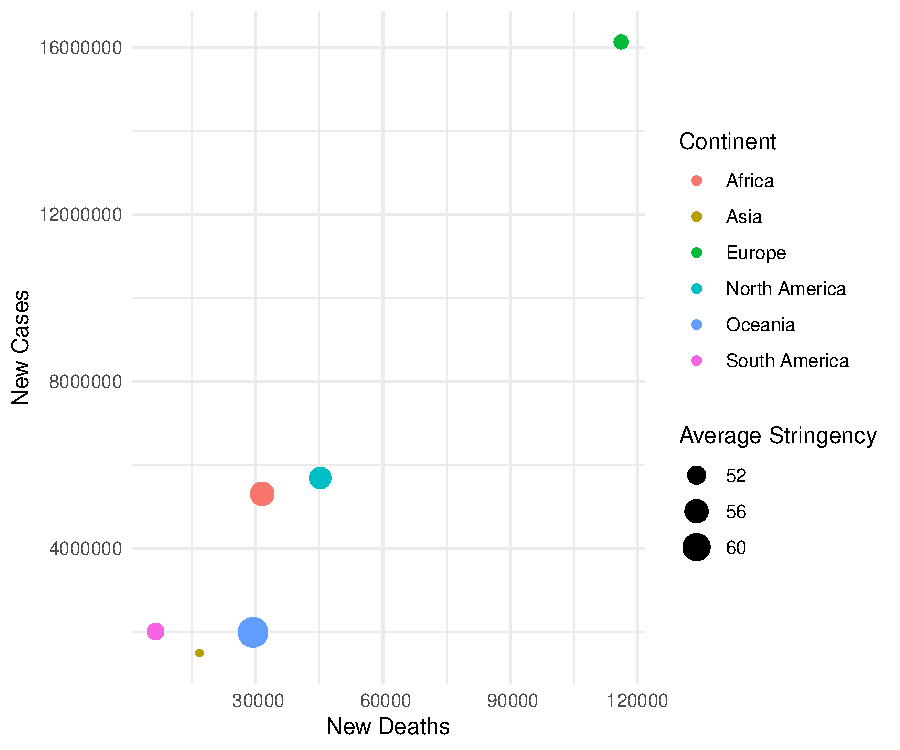
\includegraphics{Question1_files/figure-latex/unnamed-chunk-1-1.pdf}

\hypertarget{vaccination-rollout-and-gdp-per-capita}{%
\subsection{Vaccination rollout and GDP per
capita}\label{vaccination-rollout-and-gdp-per-capita}}

As expected, continents with a higher GDP per capita demonstrate a
stronger vaccination rollout per million people. However, it is
surprising to note that despite this higher vaccination rate, certain
continents (particularly Europe) still experience the highest number of
new deaths. This observation raises questions about the underlying
factors contributing to the persistently high mortality rates in these
regions, despite their comparatively stronger vaccination efforts.

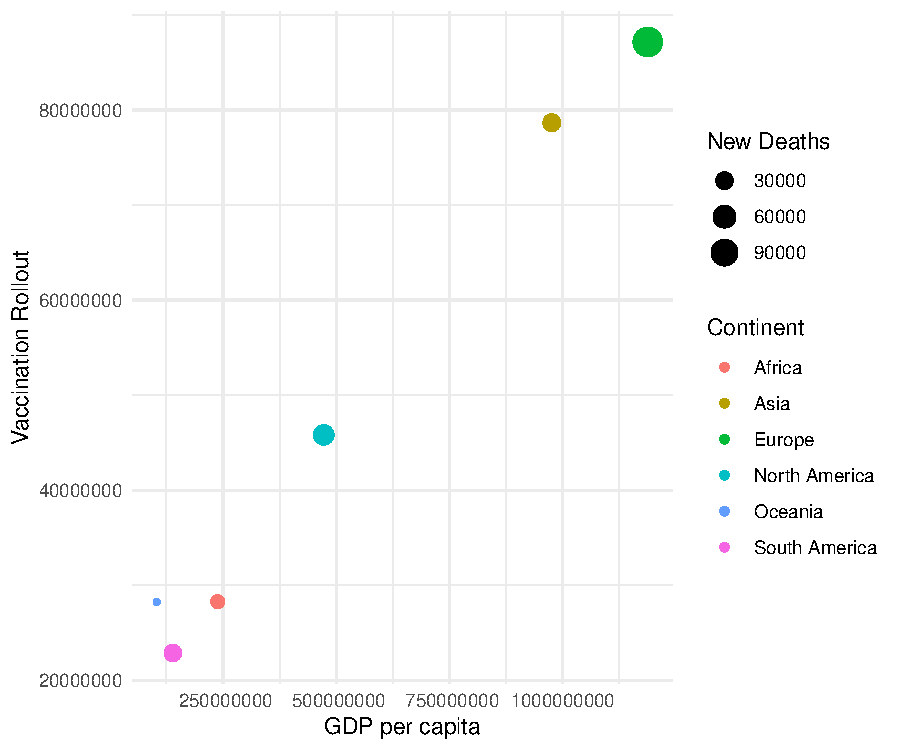
\includegraphics{Question1_files/figure-latex/unnamed-chunk-2-1.pdf}

\hypertarget{part-b}{%
\section{Part B}\label{part-b}}

In this section, I will examine two specific groups: individuals with
diabetes and smokers. Diabetes is considered a comorbidity for COVID-19
deaths, while smoking weakens lung function, which can be further
compromised by COVID-19.

Based on the graphs for both smokers and individuals with diabetes, we
observe that the statement regarding the likelihood of COVID-19-related
deaths holds true in 49.5\% of countries. This determination is made
using the median of global smoker and diabetes rates as the threshold
for the statement.

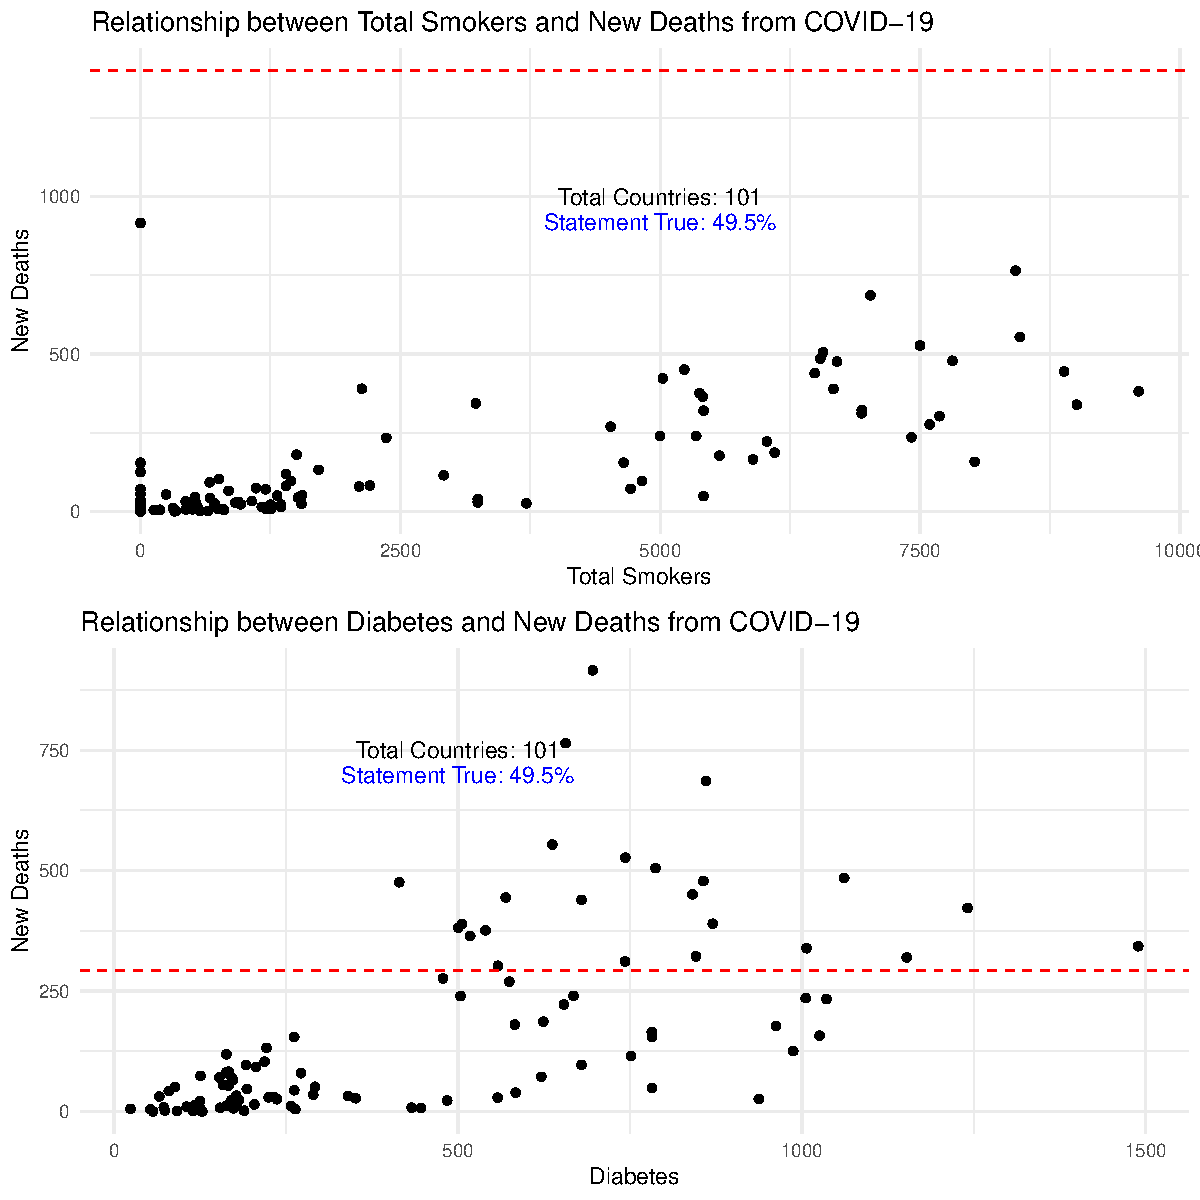
\includegraphics[angle=90]{Question1_files/figure-latex/unnamed-chunk-3-1}

\hypertarget{part-c}{%
\section{Part C}\label{part-c}}

To examine the relationship between the increase in ICU admissions and
facilities across continents, hospital beds were used as a proxy for
these facilities. The analysis focused on the number of days since the
first COVID-19 infection, with some continents excluded due to data
limitations. The graph below illustrates notable trends: Asia
demonstrates a delayed increase in facilities, occurring after
approximately 500 days since the first infection, while Europe shows an
immediate increase. In contrast, South America exhibits no noticeable
increase in facilities over time.
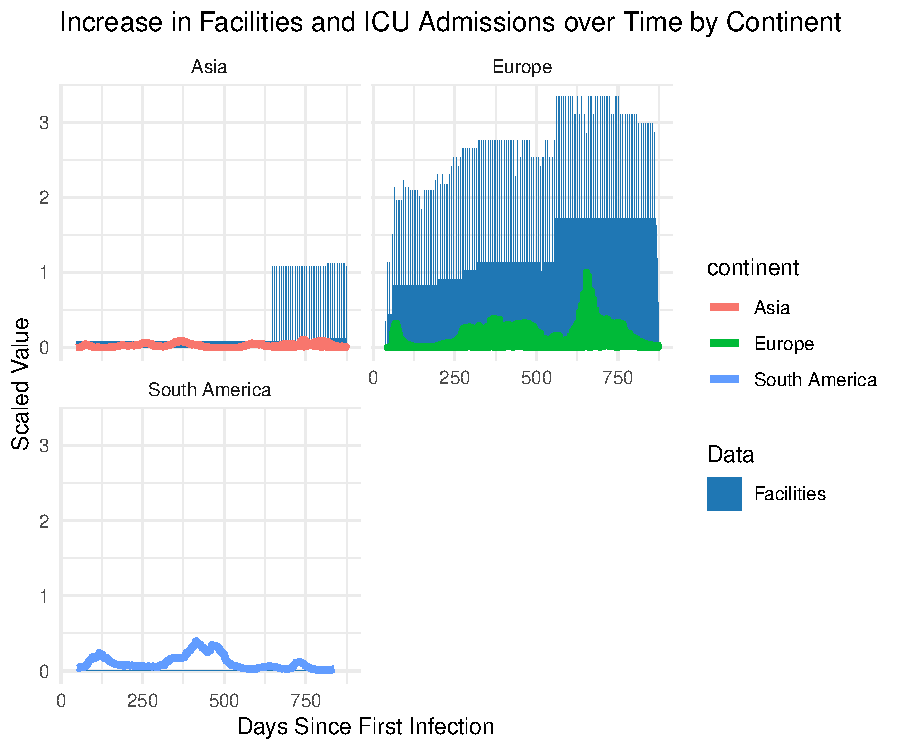
\includegraphics{Question1_files/figure-latex/unnamed-chunk-4-1.pdf}

\hfill

\hypertarget{discussion}{%
\section{Discussion}\label{discussion}}

The analysis of COVID-19 data across different regions highlights the
importance of strict lockdown measures in controlling the spread of the
virus. The observed patterns indicate that regions with higher
strictness scores tend to have lower case and death rates, while regions
with less strict measures experience higher rates of infection and
mortality. The relationship between strictness scores and outcomes can
be influenced by various factors, including population density and
healthcare system capacity.

The findings also shed light on the impact of comorbidities on COVID-19
mortality rates. Individuals with diabetes and smokers are identified as
vulnerable groups, with a higher likelihood of experiencing severe
outcomes. However, the analysis reveals that this statement holds true
only in approximately 49.5\% of countries, suggesting the presence of
additional contributing factors.

Examining the relationship between ICU admissions and facilities across
continents provides insights into the preparedness and response capacity
of healthcare systems. The delayed increase in facilities observed in
Asia and the absence of noticeable growth in South America raise
questions about the specific challenges and limitations faced by these
regions.

Overall, this analysis underscores the need for a comprehensive
understanding of various factors influencing COVID-19 outcomes. It
highlights the importance of stringent measures, considerations of
comorbidities, and the capacity of healthcare systems in managing the
pandemic effectively. Further research and investigation are necessary
to explore the specific factors contributing to the persistently high
mortality rates in certain regions, despite vaccination efforts and
other interventions.

\bibliography{Tex/ref}





\end{document}
